
%
% File: chap02.tex
% Author: Tengxiang Li
%
\chapter{Background}
\label{chap:02}
\setlength{\parskip}{1em}
%
\section{Overview}
This chapter presents a multi-dimensional evaluation of PPO, ES, and ARS, benchmarked on the Apple M1 Pro architecture. The ``Headline Result" of this study reveals a fundamental trade-off: while PPO maintains superior Sample Efficiency and consistency in serial environments, derivative-free methods—specifically Evolution Strategies (ES)—demonstrate superior Parallel Scalability. Most notably, the M1 Pro’s unified memory and multi-core efficiency allow ES to outperform PPO in high-dimensional tasks like HalfCheetah when transitioned to a distributed 4-worker configuration, highlighting a shift in algorithmic dominance when hardware resources are scaled.
\section{Continuous Control}
Continuous control refers to decision-making in environments where actions and states are real-valued rather than discrete. While the defining characteristic of continuous control lies in the action space—which is essential for generating the smooth, precise signals required for tasks like autonomous driving and legged locomotion—these problems typically involve continuous state spaces as well \citep{seif2016autonomous,smith2021legged}. Unlike discrete settings, where states and actions can often be enumerated, continuous spaces are infinite and cannot be exhaustively explored, requiring agents to learn effective control policies through direct interaction with the environment.
A major challenge in continuous control is the high dimensionality of both the state and action spaces, which leads to reduced sampling efficiency as the number of degrees of freedom increases \citep{wang2017continuous}. This phenomenon significantly complicates exploration, as the vast majority of possible state-action pairs may contribute little to actual task performance. Additionally, physical control problems often involve non-linear dynamics and discontinuous reward structures, particularly in contact-rich tasks such as locomotion, further increasing learning complexity \citep{shahid2022manipulation}.
Traditional control methods, including Proportional-Integral-Derivative (PID) and Model Predictive Control (MPC), may struggle to scale to such environments due to their dependence on accurate system models, manual tuning, or high computational constraints \citep{wang2017continuous}. These limitations have motivated the development of adaptive, learning-based approaches capable of handling the inherent uncertainty and complexity of continuous settings. To address these challenges, reinforcement learning and black-box optimization techniques have been increasingly adopted, providing alternative frameworks for policy learning without requiring explicit or differentiable system models

% \input{chapters/chapter02/section2-1}

\section{Locomotion Environments in MuJoCo}
The Multi-Joint dynamics with Contact (MuJoCo) physics engine has established itself as the definitive platform for research in continuous control and robotic locomotion. Developed to provide a balance between computational efficiency and physical accuracy, MuJoCo utilizes a unique mathematical formulation that handles complex constraints and contact dynamics through a convex optimization framework \citep{todorov2012mujoco}. This allows for the simulation of articulated systems with high degrees of freedom while maintaining the high-frequency update rates necessary for stable numerical integration.
In the context of continuous control and optimization, MuJoCo environments are utilized as standard benchmarks because they present challenges that mirror real-world physical systems. These include high-dimensional state and action spaces, non-linear system dynamics, and contact-rich interactions with the ground plane. The standardization of these tasks was originally facilitated by the OpenAI Gym framework \citep{brockman2016gym}, which has since been succeeded by the Gymnasium library \citep{towers2024gymnasium} to ensure continued maintenance and community-driven development of the benchmark suite. By utilizing these unified interfaces, the research community ensures reproducibility and maintains a common metric for evaluating the robustness and sample efficiency of various algorithmic approaches. The specific configurations and dimensional complexities of the environments used in this study are summarized in Table \ref{tab:mujoco_summary}.

\begin{table}[htbp]
    \centering
    \caption{Summary of MuJoCo Locomotion Environments and their Complexity.}
    \label{tab:mujoco_summary}
    \begin{tabular}{@{}lcccc@{}}
        \toprule
        \textbf{Environment} & \textbf{Dynamics} & \textbf{DOF} & \textbf{State Space} & \textbf{Action Space} \\ \midrule
        Hopper               & 2D Planar         & 6            & 11                   & 3                     \\
        HalfCheetah          & 2D Planar         & 9            & 17                   & 6                     \\
        Walker2d             & 2D Planar         & 9            & 17                   & 6                     \\
        Ant                  & 3D Quadruped      & 14           & 27                   & 8                     \\ \bottomrule
    \end{tabular}
\end{table}

%
\begin{figure}[htbp]
     \centering
     \begin{subfigure}[b]{0.3\textwidth} % Reduced from 0.45
         \centering
         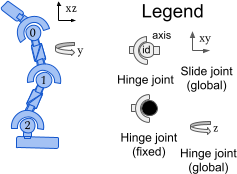
\includegraphics[width=\textwidth]{chapters/chapter02/fig02/hopper.png}
         \caption{Hopper}
         \label{fig:hopper}
     \end{subfigure}
     \hspace{1cm} % Adds controlled space between side-by-side images
     \begin{subfigure}[b]{0.3\textwidth}
         \centering
         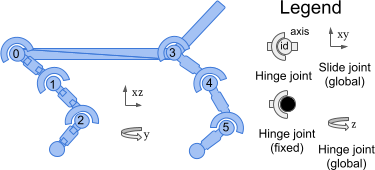
\includegraphics[width=\textwidth]{chapters/chapter02/fig02/half_cheetah.png}
         \caption{HalfCheetah}
         \label{fig:half_cheetah}
     \end{subfigure}
     
     \vspace{0.5cm} % Adds vertical space between the rows
     
     \begin{subfigure}[b]{0.3\textwidth}
         \centering
         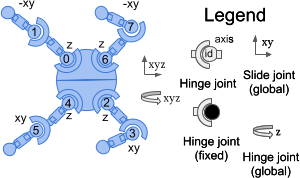
\includegraphics[width=\textwidth]{chapters/chapter02/fig02/ant.png}
         \caption{Ant}
         \label{fig:ant}
     \end{subfigure}
     \hspace{1cm}
     \begin{subfigure}[b]{0.3\textwidth}
         \centering
         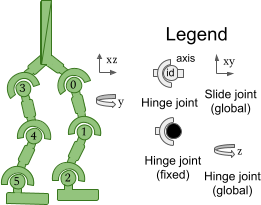
\includegraphics[width=\textwidth]{chapters/chapter02/fig02/walker2d.png}
         \caption{Walker2d}
         \label{fig:walker2d}
     \end{subfigure}
     \caption{The four MuJoCo locomotion environments used in this study. Images adapted from the Gymnasium documentation \citep{towers2024gymnasium}.}
     \label{fig:mujoco_environments}
\end{figure}
%
\subsection{The Hopper Environment}

\paragraph{Configuration and Control} 
The Hopper features a 2D planar robot (see Figure \ref{fig:hopper}) consisting of four main links: a torso, a thigh, a leg, and a foot. The primary objective is to enable this single-legged structure to hop forward along a track.

\begin{itemize}
    \item \textbf{Degrees of Freedom:} 6 (global torso position/orientation and internal hinge joints)
    \item \textbf{State Space:} 11-dimensional continuous vector (positional and velocity data)
    \item \textbf{Action Space:} 3-dimensional continuous vector (joint torques)
\end{itemize}

\paragraph{Reward Function and Objectives} 
The reward structure balances locomotion speed with stability. It is composed of a forward velocity reward, a ``healthy reward'' for remaining upright, and a control penalty to discourage excessive energy consumption. The episode terminates if the robot falls (based on torso height or tilt), forcing the agent to prioritize dynamic equilibrium alongside speed.

\paragraph{Benchmark Role} 
The Hopper is a foundational benchmark because it occupies a middle ground between simple balancing tasks and complex bipedal walking. Its inherent instability due to a single point of contact makes it an ideal testbed for evaluating the stability and gait-coordination capabilities of optimization algorithms.
%
\subsection{The HalfCheetah Environment}

\paragraph{Configuration and Control} 
The HalfCheetah is a 2D (see Figure \ref{fig:half_cheetah}) nine-link robot designed to approximate a quadruped, though constrained to a vertical plane. It includes a torso and two legs (front and back), each with a thigh, shank, and foot.

\begin{itemize}
    \item \textbf{Degrees of Freedom:} 9
    \item \textbf{State Space:} 17-dimensional continuous vector
    \item \textbf{Action Space:} 6-dimensional continuous vector (torques for all hinge joints)
\end{itemize}

\paragraph{Reward Function and Objectives} 
The primary goal is to maximize forward velocity. Unlike other tasks, the standard implementation does not terminate if the robot falls, as the torso is physically prevented from tipping over. The reward function is dominated by a forward progress term and a control cost to discourage unrealistic torque usage, allowing agents to focus purely on high-speed gait optimization.

\paragraph{Benchmark Role} 
This environment evaluates an algorithm's ability to coordinate multiple actuators for efficient cyclic gaits. Because it lacks a ``survival'' incentive, it serves as a key metric for pure locomotion speed in high-dimensional continuous spaces.
%

\subsection{The Ant Environment}

\paragraph{Configuration and Control} 
The Ant environment (Figure \ref{fig:ant}) represents a transition from 2D planar movement to 3D quadrupedal locomotion. The robot consists of a central torso and four legs, each possessing two hinge joints, resulting in a total of nine links. Because the agent can move in any direction on the XY-plane, the complexity is significantly higher than 2D benchmarks.

\begin{itemize}
    \item \textbf{Degrees of Freedom:} 14 (6 for the free-joint torso and 8 for the hip and knee hinges)
    \item \textbf{State Space:} Approximately 27-dimensional (including torso orientation, joint positions, and velocities)
    \item \textbf{Action Space:} 8-dimensional continuous vector (motor torques for the four limbs)
\end{itemize}

\paragraph{Reward Function and Objectives} 
The objective is to move forward as quickly as possible while maintaining a stable torso height. The reward function includes a velocity term and a healthy reward, balanced by a control penalty to discourage jerky movements and energy waste. Contact penalties are often included to prevent the legs from exerting unrealistic forces on the ground. The structure encourages the emergence of a stable quadrupedal gait that can navigate the 3D environment without flipping or colliding its torso with the floor.

\paragraph{Benchmark Role} 
The Ant is a staple in continuous control research because it tests an algorithm's scalability to 3D dynamics and high-dimensional action spaces. Its complex limb interactions and the requirement for coordination across four independent actuators make it a standard benchmark for evaluating exploratory capabilities and robustness of modern optimization frameworks in multi-directional locomotion.
%
\subsection{The Walker2d Environment}

\paragraph{Configuration and Control} 
The Walker2d (Figure \ref{fig:walker2d}) features a bipedal robot with seven links: a torso and two symmetric legs (thighs, legs, and feet), restricted to a 2D plane.

\begin{itemize}
    \item \textbf{Degrees of Freedom:} 9
    \item \textbf{State Space:} 17-dimensional continuous vector
    \item \textbf{Action Space:} 6-dimensional continuous vector (torques for both legs)
\end{itemize}

\paragraph{Reward Function and Objectives} 
The multi-faceted reward emphasizes forward locomotion, stability, and energy efficiency. It includes a velocity reward, a survival (healthy) reward, and a penalty for action magnitude. The episode terminates if the torso height falls below a threshold or tilts excessively, necessitating a balance between speed and bipedal stability.

\paragraph{Benchmark Role} 
The Walker2d is significantly more challenging than the Hopper due to the requirement for alternating limb coordination. It is a standard benchmark for testing how agents handle contact transitions between two feet, serving as a precursor to 3D humanoid locomotion.
%


\section{Optimization Approaches}
Optimization is the process of identifying input configurations that produce a desired outcome within a given model \citep{eiben2015ec}. Objectives may be defined explicitly, where a fixed target value is specified, or implicitly, where solutions are evaluated relative to one another rather than against a predetermined threshold. In implicit optimization, the goal is to discover the best achievable performance—such as minimizing a path length—among all feasible candidates.
In continuous control settings, optimization typically involves iteratively refining policy parameters to maximize a reward signal. This process is commonly approached through two main paradigms: gradient-based methods, such as Deep Reinforcement Learning, which exploit gradient information to guide parameter updates, and Black-Box Optimization, which treats the system as opaque and relies on stochastic search and repeated function evaluations to identify effective behaviors.

\subsection{Deep Reinforcement Learning (DRL)}

Reinforcement learning (RL) \citep{sutton2018rl} represents an essential direction within the field of machine learning, aiming to enable an autonomous agent to learn an optimal policy through iterative interactions with an environment. Unlike supervised learning, which relies on static labeled datasets, RL is dynamic, aiming to maximize a numerical reward signal over time. \textbf{Deep reinforcement learning (DRL)} extends this framework by utilizing deep neural networks as function approximators, allowing the agent to map high-dimensional sensory inputs to optimal actions \citep{zai2020drlaction} (see Figure~\ref{fig:drl}). By utilizing neural networks as function approximators, the agent can generalize experiences across vast state spaces—a capability that was historically limited by the constraints of tabular RL methods.

\begin{figure}[h!]
    \centering
    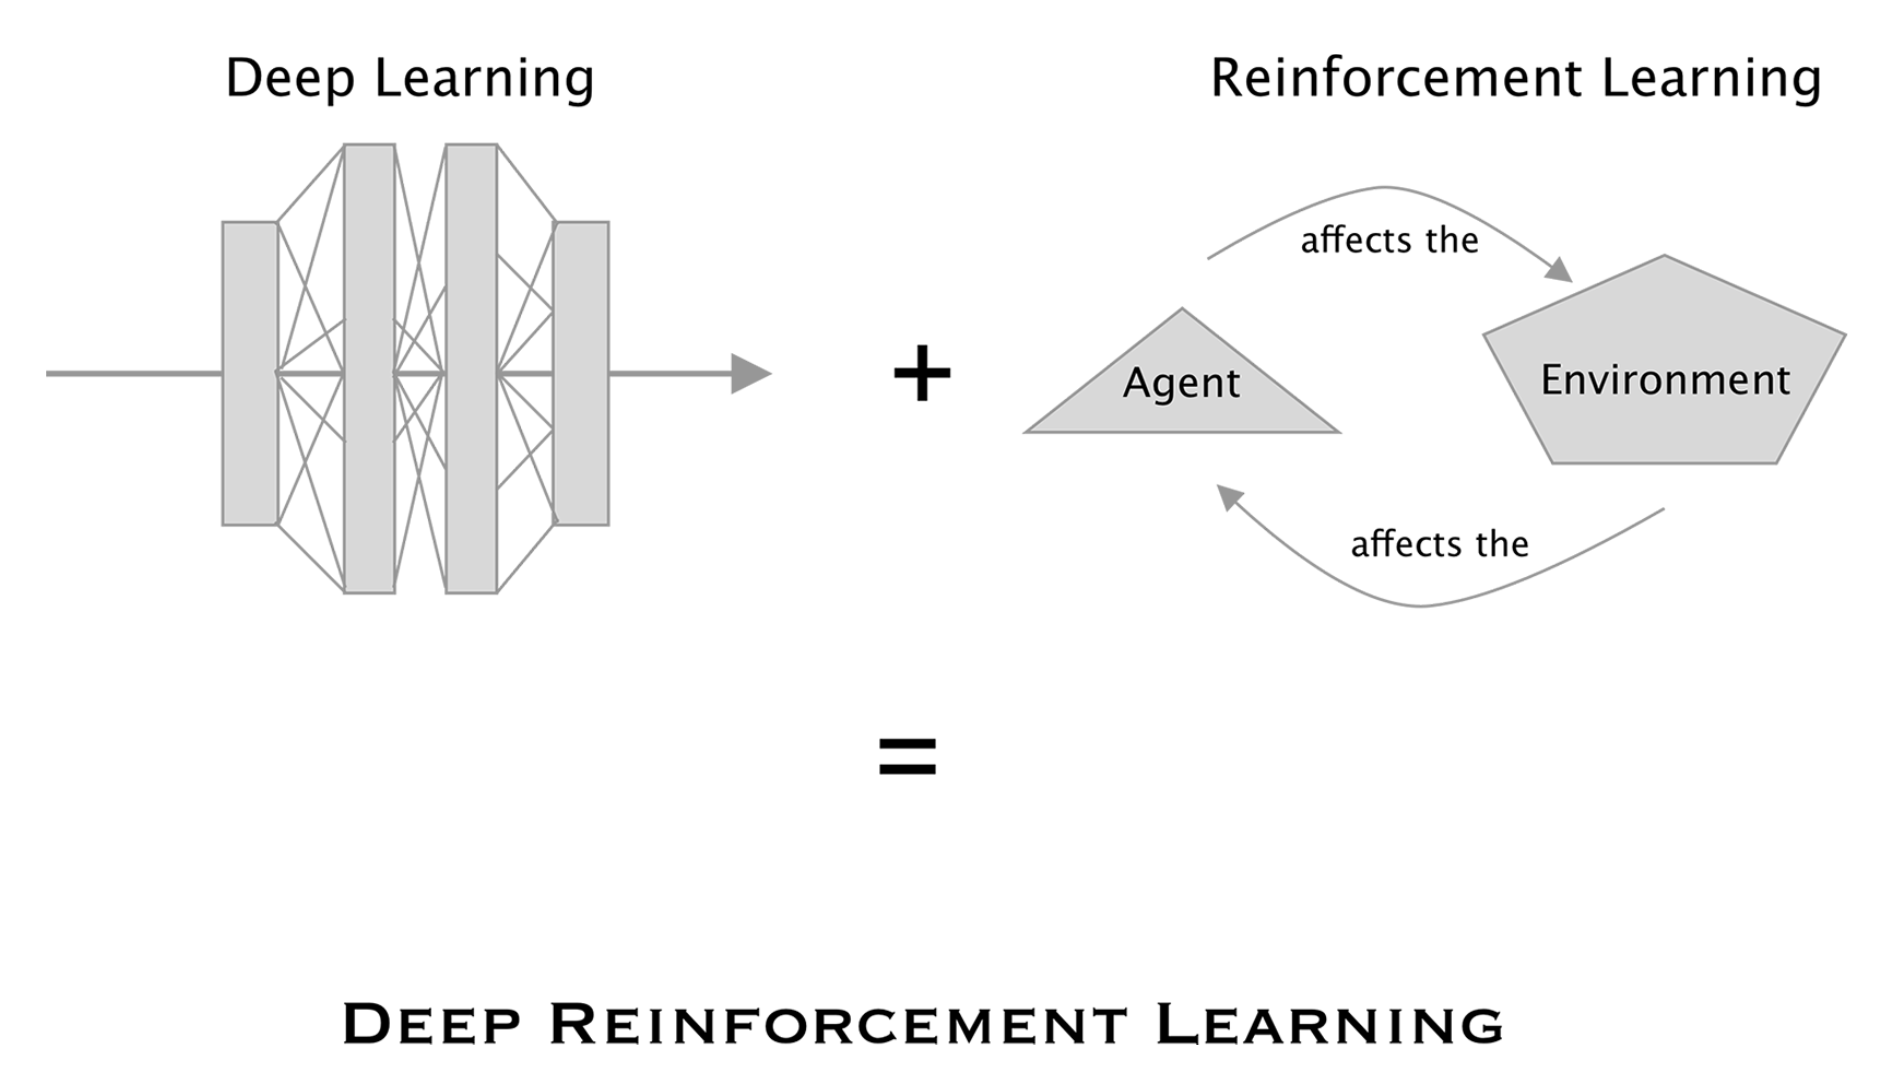
\includegraphics[width=0.7\textwidth]{logos/dl.png}
    \caption{The conceptual intersection of Deep Reinforcement Learning, combining the function approximation power of Deep Learning with the goal-oriented behavior of Reinforcement Learning \citep{zai2020drlaction}.}
    \label{fig:drl}
\end{figure}

The DRL framework operates as a Markov Decision Process (MDP) \citep{bellman1957dp}, typically defined by the tuple $(\mathcal{S}, \mathcal{A}, P, R, \gamma)$. In this setting, the agent observes a state $s_t \in \mathcal{S}$ and selects an action $a_t \in \mathcal{A}$. The environment then responds by transitioning to a new state $s_{t+1}$ according to the transition distribution $P(s_{t+1}|s_t, a_t)$ and providing a scalar reward $r_t = R(s_t, a_t)$. The primary goal of the agent is to identify a policy $\pi$ that maximizes the expected return $G_t$, representing the cumulative discounted rewards:

\begin{equation} \label{eq:return}
V^\pi(s) = \mathbb{E}_\pi \left[ \sum_{t=0}^{\infty} \gamma^t r_t \mid s_0 = s \right],
\end{equation}

where $\gamma$ is the discount factor that weights immediate versus future rewards.

In the literature, RL approaches are broadly categorized into two branches: \textbf{model-based} and \textbf{model-free}. \textbf{Model-based} methods attempt to learn the transition dynamics $P$ and reward function $R$ to simulate the environment. In contrast, \textbf{model-free} methods—which are the focus of this work—learn the policy or value function directly from experience without attempting to model the underlying environment physics.

\subsubsection{Value-Based and Policy Search Methods}

Within the \textbf{model-free} regime, the policy can be derived from learned value functions or optimized directly through policy search. Value-based methods focus on approximating the state-action value function $Q(s,a)$, which predicts the expected cumulative rewards and satisfies the Bellman equation \citep{bellman1957dp}:

\begin{equation} \label{eq:bellman}
Q^\pi(s, a) = R(s, a) + \gamma \mathbb{E}_{s' \sim P(\cdot|s,a)} [V^\pi(s')],
\end{equation}

where $Q(s,a)$ is referred to as the value function. Once obtained, a policy may be derived by selecting the action with the highest value:

\begin{equation} \label{eq:policy_from_q}
\pi(s_t) = \arg\max_a Q(s_t, a).
\end{equation}

However, value-based methods can face challenges such as policy degradation, leading researchers toward direct policy search. In this approach, the policy $\pi_\theta$ acts as a direct controller and may be deterministic—mapping a specific action to a state—or stochastic, defining a probability distribution over actions. While deterministic policies often require parameter perturbation for exploration, stochastic policies inherently address the exploration-exploitation dilemma by sampling diverse actions. In continuous problems, stochastic policies frequently employ Gaussian distributions to handle infinite action spaces:

\begin{equation} \label{eq:stochastic_policy}
\pi_\theta(a|s) = \frac{1}{\sqrt{2\pi}\sigma} \exp\left( -\frac{(a - h_\theta(s))^2}{2\sigma^2} \right),
\end{equation}

where $h_\theta(s)$ represents a neural network with parameters $\theta$. To optimize this architecture, Policy Gradient methods are employed \citep{peters2010policy}. Because this parametric model is differentiable, the agent can optimize the parameters $\theta$ to maximize the expected return $J(\theta)$ by following the policy gradient:

\begin{equation} \label{eq:policy_gradient}
\nabla_\theta J(\theta) = \mathbb{E}_{\pi_\theta} [\nabla_\theta \ln \pi_\theta(a|s) A^\pi(s, a)].
\end{equation}

\subsubsection{Actor-Critic Architectures and Stability}

To leverage the strengths of both paradigms, \textbf{Actor-Critic} methods \citep{konda1999actorcritic} employ a dual-structure architecture. The \textbf{Actor} serves as the policy-based component, while the \textbf{Critic} estimates the state-value function $V(s)$. This evaluation is often expressed through the advantage function $A(s, a) = Q(s, a) - V(s)$, which measures how much better a specific action is compared to the average return from that state.

In practice, since$Q(s, a)$ is often unknown, the advantage is approximated using the Temporal Difference (TD) error \citep{sutton1988td}. By utilizing the critic’s value estimates for bootstrapping—updating the current estimate based on the predicted value of the next state—the agent can perform online updates via the TD error:

\begin{equation} \label{eq:td_error}
V^\pi(s_t) \leftarrow V^\pi(s_t) + \delta \cdot [r_t + \gamma V^\pi(s_{t+1}) - V^\pi(s_t)],
\end{equation}

where $\delta_t$ denotes the step size. This mechanism allows the agent to learn incrementally from partial sequences  (step-by-step) rather than waiting for an entire episode to conclude, as required by Monte Carlo methods like REINFORCE \citep{williams1992reinforce}. Unlike REINFORCE, which sums all rewards until the terminal state and thus introduces high variance, TD learning significantly improves sample efficiency by making updates at every time step based on learned estimates.

Despite these advancements, achieving stability in high-dimensional continuous control remains a significant challenge, as a single suboptimal gradient update can lead to a destructive policy change and performance collapse. Consequently, modern DRL research has focused on stabilizing these updates through techniques such as Generalized Advantage Estimation (GAE) \citep{schulman2016gae}, which reduces variance by taking a weighted average of $n$-step advantage estimators. These advancements, alongside trust-region and clipping constraints found in algorithms such as A2C, TRPO, and PPO \citep{mnih2016a3c,schulman2015trpo,schulman2017ppo}, provide the foundation for the robust performance required in complex locomotion tasks.

\subsection{Black-Box Optimization}

Black-box optimization refers to the process of optimizing a system where the internal computational mechanisms or underlying models are not explicitly defined or accessible. In such scenarios, the optimizer provides an input and receives an output through a process in which only objective function evaluations—often referred to as a fitness or cost value—are available to guide the search \citep{eiben2015ec}. This paradigm is particularly effective for complex real-world problems in domains such as healthcare, scientific discovery, aeronautical design, and control, where direct analytical modeling is frequently infeasible.

Over several decades, black-box optimization algorithms have demonstrated the ability to produce high-quality or near-optimal solutions for problems that would otherwise require extensive manual tuning by domain experts \citep{wierstra2011nes}. Their success stems from their flexibility and robustness when dealing with noisy, high-dimensional, or poorly understood systems, making them well suited for modern optimization challenges where transparency of the underlying process cannot be assumed.

\subsection{Derivative-Free Optimization (DFO)}

Derivative-free optimization (DFO), also known as zeroth-order or black-box optimization, comprises a class of algorithms that do not rely on gradient information to navigate the search space. Instead, these methods operate exclusively on observed function values $f(x)$ obtained by evaluating candidate solutions $x$ \citep{conn2009dfo,kolda2003directsearch,rios2013derivativefree}. This characteristic makes DFO particularly attractive for optimization problems where gradients are unavailable, unreliable, or computationally expensive to obtain.

As discussed in Section~2.2, objective functions arising in complex continuous control tasks—especially those involving contact dynamics—are often non-convex, non-smooth, or even discontinuous. In such settings, gradient-based methods may suffer from vanishing gradients or become trapped in suboptimal local minima. DFO methods address these challenges by directly exploring the search space through iterative sampling strategies, rather than relying on local derivative information.

The general framework of DFO algorithms follows a structured iterative cycle. The process typically begins with the random sampling of initial candidate solutions within the search space. Based on the evaluated fitness values, the algorithm constructs an explicit or implicit model of the objective function to identify promising regions for improvement. New candidate solutions are then sampled according to this model, evaluated, and used to update the model accordingly. This sampling-and-updating loop continues until a predefined termination condition is met, such as exhausting the evaluation budget or achieving a satisfactory objective value.

Because DFO methods do not impose differentiability constraints on the objective function, they are highly versatile and can be applied to continuous, discrete, or mixed-variable optimization problems. This flexibility has made derivative-free optimization a foundational tool in modern black-box optimization and a strong alternative to gradient-based approaches in challenging control and learning environments.

\subsubsection{Random Search}

Within the taxonomy of derivative-free optimization, \textit{Random Search}—often categorized as stochastic zeroth-order optimization—represents one of the most fundamental yet effective approaches. Unlike more sophisticated algorithms that maintain explicit models of the objective landscape, random search identifies new candidate solutions through stochastic perturbations of the current best-known parameters or by uniformly sampling the search space.

Despite its simplicity, random search has received considerable attention in the context of continuous control. Empirical studies have shown that such methods can achieve competitive performance when compared to gradient-based reinforcement learning algorithms, particularly when optimizing static or linear policies for MuJoCo locomotion benchmarks such as the Hopper environment discussed in Section~2.3 \citep{mania2018randomsearch}. These findings challenge the assumption that gradient information is always necessary for effective policy optimization in high-dimensional continuous spaces.

The convergence behavior and theoretical properties of zeroth-order random search methods have been progressively analyzed, demonstrating that they can serve as strong and reliable baselines for black-box optimization. While random search itself lacks mechanisms for structured exploration or population-level diversity, it provides a conceptual foundation upon which more advanced derivative-free optimization techniques are built. In particular, population-based approaches—most notably those found in evolutionary computing—extend this paradigm to enhance exploration and global optimization capabilities.

\subsubsection{Evolutionary Computing (EC)}

Evolutionary Computing (EC) constitutes a major subclass of derivative-free optimization and black-box optimization techniques inspired by the principles of natural evolution. Within this framework, the optimization problem is analogized to a natural environment, candidate solutions are treated as individuals, and their quality is evaluated using a fitness function. Through iterative cycles of variation and selection, EC algorithms progressively improve the fitness of a population, approximating optimal solutions over successive generations.

Historically, the field of evolutionary computation emerged in the 1960s through three independent research streams: evolutionary programming, genetic algorithms, and evolution strategies. Although these approaches developed largely in isolation for several decades, they were later unified under the broader discipline of evolutionary computing. Today, these methodologies—alongside later developments such as genetic programming—form a cohesive family of algorithms designed to address complex optimization problems in a robust and automated manner \citep{eiben2015ec}.

\paragraph{Evolution Strategies (ES)}

Evolution Strategies were originally developed to address optimization problems in high-dimensional, continuous-valued search spaces \citep{rechenberg1973evolutionsstrategie,schwefel1977numerical}. In contrast to evolutionary methods that rely on discrete representations, ES typically encode candidate solutions as real-valued parameter vectors. This representation makes them particularly well suited for neuroevolution, where neural network parameters such as weights and biases are directly optimized without gradient information \citep{risi2017neuroevolution}.

The canonical ES framework operates on a population of parameter vectors, often referred to as genotypes. During each generation, offspring are generated by applying stochastic perturbations to the parent solutions. These offspring are evaluated using the objective function, and selection mechanisms retain the highest-performing individuals to form the next generation. This iterative process enables the algorithm to gradually refine solutions through exploration and selection \citep{pagliuca2018}.

A significant advancement within this family is the \textit{Covariance Matrix Adaptation Evolution Strategy} (CMA-ES) \citep{hansen2001cmaes}. Unlike simpler ES variants that apply isotropic noise, CMA-ES maintains a multivariate Gaussian distribution over the parameter space. By adaptively estimating and updating the covariance matrix, the algorithm captures correlations between parameters and directs the search toward promising directions. This property makes CMA-ES particularly effective for optimizing low- to medium-dimensional continuous problems, where parameter interactions play a critical role in performance.

\subsubsection{Natural Evolution Strategies (NES)}

Natural Evolution Strategies (NES) \citep{wierstra2014nes} represent a more theoretically principled evolution of the black-box optimization framework. Unlike traditional ES, which maintains a discrete population of search points, NES maintains and updates a parameterized search distribution, $p_\theta(x)$, over the set of candidate solutions $x$. The objective is to maximize the expected fitness $\mathbb{E}_{x \sim p_\theta}[f(x)]$ under this distribution:

\begin{equation}
J(\theta) = \mathbb{E}_{x \sim p_\theta}[f(x)].
\end{equation}

The core innovation of NES is the use of the natural gradient to update the distribution parameters $\theta$. The gradient of the expected fitness is estimated using the score function estimator:

\begin{equation}
\nabla_\theta J(\theta) = \mathbb{E}_{x \sim p_\theta} \big[ f(x)\nabla_\theta \log p_\theta(x) \big].
\end{equation}

To compute the natural gradient update, the vanilla gradient is adjusted by the inverse of the Fisher Information Matrix $F$, which represents the local curvature of the parameter space:

\begin{equation}
\tilde{\nabla}_\theta J(\theta) = F^{-1} \nabla_\theta J(\theta).
\end{equation}

The parameters are updated in the direction of the natural gradient:

\begin{equation}
\theta \leftarrow \theta + \eta \tilde{\nabla}_\theta J(\theta),
\end{equation}

where $\eta$ denotes the learning rate.

By following the natural gradient, NES ensures that updates are invariant to the parameterization of the distribution and prevents the premature convergence often seen in plain gradient methods. The NES family includes variations designed to balance computational efficiency with search accuracy, such as Exponential NES (xNES) for modeling complex dependencies and Separable NES (sNES) for scaling to significantly larger search spaces. By deriving updates from first principles, NES provides a mathematically grounded foundation for the iterative optimization of complex, high-dimensional functions.

\subsection{Summary}

This chapter established the fundamental concepts and benchmarking environments necessary for this research. The key takeaways are summarized below:

\begin{itemize}
    \item \textbf{Continuous Control Challenges:} Real-valued state and action spaces require adaptive learning due to their high dimensionality and complex contact dynamics.
    \item \textbf{Standardized Benchmarking:} The MuJoCo physics engine provides a suite of locomotion tasks that serve as common metrics for evaluating algorithmic robustness.
    \item \textbf{Optimization Paradigms:} Two distinct approaches were identified for policy learning:
    \begin{itemize}
        \item \textbf{Deep Reinforcement Learning (DRL):} A gradient-based framework utilizing neural networks to maximize cumulative rewards.
        \item \textbf{Black-Box Optimization:} A gradient-free paradigm relying on:
        \begin{itemize}
            \item \textbf{Derivative-Free Optimization (DFO):} Zero-order algorithms that navigate search spaces using only function evaluations.
            \item \textbf{Random Search:} A fundamental DFO method using stochastic parameter perturbations.
            \item \textbf{Evolutionary Computing:} Population-based methods, including Evolution Strategies (ES) and Natural Evolution Strategies (NES), which adapt search distributions through selection and mutation.
        \end{itemize}
    \end{itemize}
\end{itemize}

By establishing these theoretical and environmental foundations, this chapter prepares the necessary context for the methodology and experimental evaluations that follow.

\clearpage
\null % creates an empty page
\clearpage